% =====================================================================
%  OPERACIÓN FOGÓN · PHP desde cero · presentación de clase (3 horas)
%  Tecnología Web I · UPDS Tarija · FORJA WEB 2026
%  M.Sc. Ing. Juan Pablo Cruz Ovando · jpcruzovando.com
%  Compilar:  lualatex fogon-presentacion.tex   (2 veces)
% =====================================================================
\documentclass[aspectratio=169,11pt]{beamer}
\usepackage{fontspec}
\usepackage{polyglossia}
\setdefaultlanguage{spanish}
\usepackage{tikz}
\usetikzlibrary{positioning,arrows.meta,calc,shapes.geometric,shadows,fit,backgrounds}
\usepackage{listings}
\usepackage[most]{tcolorbox}
\usepackage{tabularx,booktabs,array}

% ---------------- Fuentes ----------------
\IfFontExistsTF{Fira Sans}{%
  \setsansfont{Fira Sans Light}[BoldFont={Fira Sans SemiBold}]
  \newfontfamily\titular{Fira Sans Black}
  \newfontfamily\medio{Fira Sans Medium}}{%
  \setsansfont{TeX Gyre Heros}
  \newfontfamily\titular{TeX Gyre Heros}[UprightFont=*-Bold]
  \newfontfamily\medio{TeX Gyre Heros}}
\setmonofont{DejaVu Sans Mono}[Scale=0.86]
\newfontfamily\simbolos{DejaVu Sans}

% ---------------- Paleta FUEGO ----------------
\definecolor{negro}{HTML}{0B0807}
\definecolor{panel}{HTML}{1A1310}
\definecolor{linea}{HTML}{2E2019}
\definecolor{fuego}{HTML}{FF7A18}
\definecolor{brasa}{HTML}{FF3D2E}
\definecolor{oro}{HTML}{FFC93C}
\definecolor{cian}{HTML}{00E5FF}
\definecolor{verde}{HTML}{39FF88}
\definecolor{lila}{HTML}{B48CFF}
\definecolor{rojo}{HTML}{FF3D5A}
\definecolor{texto}{HTML}{F6ECE4}
\definecolor{gris}{HTML}{A8968A}

\setbeamercolor{background canvas}{bg=negro}
\setbeamercolor{normal text}{fg=texto,bg=negro}
\setbeamercolor{structure}{fg=fuego}
\setbeamercolor{alerted text}{fg=brasa}
\setbeamertemplate{navigation symbols}{}
\setbeamertemplate{itemize item}{\color{fuego}\simbolos\small ▸}
\setbeamertemplate{itemize subitem}{\color{oro}\simbolos\scriptsize ▹}
\setbeamertemplate{enumerate item}{\color{fuego}\ttfamily\insertenumlabel.}

% ---------------- HUD ----------------
\newcommand{\hud}{OPERACIÓN FOGÓN}
\setbeamertemplate{background}{%
  \begin{tikzpicture}[remember picture,overlay]
    \fill[negro] (current page.south west) rectangle (current page.north east);
    \shade[top color=fuego!22!negro,bottom color=negro,opacity=0.9] ($(current page.south west)+(0,0)$) rectangle ($(current page.south east)+(0,1.6)$);
    \foreach \x in {0,0.8,...,16.4}{\draw[linea,line width=0.25pt,opacity=0.5] ($(current page.south west)+(\x,0)$) -- ++(0,9);}
    \foreach \y in {0,0.8,...,9.2}{\draw[linea,line width=0.25pt,opacity=0.5] ($(current page.south west)+(0,\y)$) -- ++(16.1,0);}
    \draw[fuego,line width=1.2pt] ($(current page.north west)+(0.25,-0.75)$) -- ++(0,0.5) -- ++(0.5,0);
    \draw[fuego,line width=1.2pt] ($(current page.north east)+(-0.25,-0.75)$) -- ++(0,0.5) -- ++(-0.5,0);
    \draw[oro,line width=1.2pt] ($(current page.south west)+(0.25,0.75)$) -- ++(0,-0.5) -- ++(0.5,0);
    \draw[oro,line width=1.2pt] ($(current page.south east)+(-0.25,0.75)$) -- ++(0,-0.5) -- ++(-0.5,0);
    \node[anchor=south west,text=gris,font=\ttfamily\tiny] at ($(current page.south west)+(0.9,0.22)$) {// \hud};
    \node[anchor=south east,text=gris,font=\ttfamily\tiny] at ($(current page.south east)+(-0.9,0.22)$) {UPDS TARIJA · TECNOLOGÍA WEB I · \insertframenumber};
  \end{tikzpicture}}

\setbeamertemplate{frametitle}{%
  \vspace{4mm}%
  {\ttfamily\scriptsize\color{fuego}// \hud}\\[-0.5mm]
  {\titular\LARGE\color{texto}\insertframetitle}%
  \ifx\insertframesubtitle\empty\else\\[-0.5mm]{\small\color{oro}\insertframesubtitle}\fi
  \par\vspace{-1mm}}
\setbeamertemplate{footline}{}

% ---------------- Efecto fuego (glitch cálido) ----------------
\newcommand{\glitch}[4][west]{%
  \node[anchor=#1,text=brasa,opacity=0.9,font=\titular#3] at ($(#2)+(-0.07,0.04)$) {#4};
  \node[anchor=#1,text=oro,opacity=0.85,font=\titular#3] at ($(#2)+(0.07,-0.04)$) {#4};
  \node[anchor=#1,text=white,font=\titular#3] at (#2) {#4};}

% Llamas decorativas
\newcommand{\llamas}[2]{% x y (desde el centro)
  \foreach \i/\h/\c in {0/1.0/brasa,0.35/1.45/fuego,0.7/1.1/oro,1.05/1.6/fuego,1.4/0.9/brasa,1.75/1.3/oro}{
    \fill[\c,opacity=0.85] ($(current page.center)+(#1+\i,#2)$) .. controls +(0.05,0.4*\h) and +(-0.1,-0.3*\h) .. ++(0.12,\h)
      .. controls +(0.08,-0.4*\h) and +(0.05,0.35*\h) .. ++(0.18,-\h) -- cycle;}}

% ---------------- Portada de nivel ----------------
\newcommand{\nivel}[5]{%
  \renewcommand{\hud}{NIVEL #1 · #2}%
  \begin{frame}[plain]
  \begin{tikzpicture}[remember picture,overlay]
    \coordinate (R) at ($(current page.center)+(4.6,0)$);
    \foreach \r in {0.8,1.6,2.4,3.2,4.0}{\draw[#4,opacity=0.22,line width=0.6pt] (R) circle (\r);}
    \fill[#4,opacity=0.13] (R) -- ++(10:4) arc (10:70:4) -- cycle;
    \draw[#4,line width=1.4pt,opacity=0.9] (R) -- ++(70:4);
    \node[text=#4,opacity=0.13,font=\titular\fontsize{190}{190}\selectfont] at ($(R)+(0.2,-0.2)$) {#1};
    \node[anchor=west,text=#4,font=\ttfamily\normalsize] at ($(current page.west)+(1,1.75)$) {>\,NIVEL #1 · ENCENDIENDO EL FUEGO\ldots};
    \coordinate (T) at ($(current page.west)+(0.95,0.55)$);
    \glitch{T}{\fontsize{44}{48}\selectfont}{#2}
    \node[anchor=north west,text=texto,font=\large,text width=8.4cm] at ($(current page.west)+(1,-0.35)$) {#3};
    \fill[linea] ($(current page.west)+(1,-2.2)$) rectangle ++(6,0.18);
    \fill[#4] ($(current page.west)+(1,-2.2)$) rectangle ++({6*#5},0.18);
    \node[anchor=west,text=gris,font=\ttfamily\tiny] at ($(current page.west)+(7.15,-2.11)$) {\pgfmathparse{int(100*#5)}\pgfmathresult\%};
  \end{tikzpicture}
  \end{frame}}

\newcommand{\impacto}[2][texto]{%
  \begin{frame}[plain]
  \begin{tikzpicture}[remember picture,overlay]
    \node[align=center,text width=14.4cm,text=#1,font=\titular\fontsize{27}{33}\selectfont] at (current page.center) {#2};
  \end{tikzpicture}
  \end{frame}}

% ---------------- Cajas ----------------
\newtcolorbox{carta}[2][fuego]{enhanced, colback=panel, colframe=#1, coltext=texto, arc=2mm, boxrule=1pt,
  left=2.5mm, right=2.5mm, top=1.5mm, bottom=1.5mm, fontupper=\small,
  title={\medio #2}, coltitle=negro, colbacktitle=#1, fonttitle=\small, borderline={0.4pt}{1.2pt}{#1!35}}
\newtcolorbox{dato}[1][fuego]{enhanced, colback=panel, colframe=#1, coltext=texto, arc=1.5mm, boxrule=0pt,
  leftrule=3pt, left=3mm, right=3mm, top=1.5mm, bottom=1.5mm, fontupper=\small}

% ---------------- Código PHP con color ----------------
\lstdefinestyle{php}{basicstyle=\ttfamily\footnotesize\color{texto}, breaklines=true, columns=fullflexible, keepspaces=true,
  showstringspaces=false, upquote=true, aboveskip=0pt, belowskip=0pt,
  alsoletter={\$}, keywordsprefix={\$}, morekeywords=[1]{zzzdummy}, keywordstyle=[1]{\color{cian}},
  morekeywords=[2]{echo,if,else,elseif,foreach,as,endforeach,endif,require,function,return,new,try,catch,true,false,count,date,isset},
  keywordstyle={[2]\color{fuego}\bfseries},
  morestring=[b]', morestring=[b]", stringstyle=\color{oro},
  morecomment=[l]{//}, commentstyle=\color{gris}\itshape,
  literate={á}{{á}}1 {é}{{é}}1 {í}{{í}}1 {ó}{{ó}}1 {ú}{{ú}}1 {ñ}{{ñ}}1 {¿}{{¿}}1 {¡}{{¡}}1 {→}{{\simbolos→}}1}
\lstset{style=php}
\newtcblisting{codigo}[2][fuego]{enhanced, listing only, colback=black, colframe=#1, arc=1.5mm, boxrule=0.8pt,
  left=2.5mm, right=2.5mm, top=1mm, bottom=1mm,
  title={\ttfamily\scriptsize\textcolor{rojo}{\simbolos●}\textcolor{oro}{\simbolos●}\textcolor{verde}{\simbolos●}\hspace{2mm}#2},
  coltitle=#1, colbacktitle=black, toptitle=0.5mm, bottomtitle=0.3mm, titlerule=0.4pt,
  borderline={0.4pt}{1pt}{#1!30}, listing options={style=php}}

\tikzset{invisible/.style={opacity=0,text opacity=0},
  visible on/.style={alt={#1{}{invisible}}},
  alt/.code args={<#1>#2#3}{\alt<#1>{\pgfkeysalso{#2}}{\pgfkeysalso{#3}}},
  caja/.style={draw=#1,fill=panel,rounded corners=1.5mm,line width=1pt,text=texto,align=center,font=\small,minimum height=1.1cm},
  flecha/.style={-{Stealth[length=2.6mm]},line width=1.2pt,#1},
  chip/.style={fill=#1,text=negro,rounded corners=1mm,font=\ttfamily\bfseries\scriptsize,inner sep=2.5pt}}

\newcommand{\demo}[1]{\begin{tikzpicture}[remember picture,overlay]
  \node[anchor=north east,fill=brasa,text=white,font=\ttfamily\bfseries\scriptsize,rounded corners=1mm,inner sep=4pt] at ($(current page.north east)+(-0.9,-0.45)$) {\simbolos●\ #1};
  \end{tikzpicture}}

\newcommand{\captura}[2][12.4cm]{\begin{tikzpicture}\node[draw=fuego!60,line width=0.8pt,rounded corners=1mm,inner sep=0pt]{\includegraphics[width=#1]{#2}};\end{tikzpicture}}

\begin{document}

% #####################################################################
%  APERTURA
% #####################################################################
\renewcommand{\hud}{TRANSMISIÓN ENTRANTE}
\begin{frame}[plain]
  \begin{tikzpicture}[remember picture,overlay]
    \node[anchor=west,text=oro,font=\ttfamily\large] at ($(current page.west)+(1.2,1.6)$) {> dos páginas. mismo diseño. misma URL\ldots};
    \coordinate (T) at ($(current page.west)+(1.15,0.3)$);
    \glitch{T}{\fontsize{36}{40}\selectfont}{Una sabe qué hora es.}
    \only<2>{\coordinate (T2) at ($(current page.west)+(1.15,-1.2)$);
      \node[anchor=west,text=brasa,font=\titular\fontsize{36}{40}\selectfont] at (T2) {La otra, no.};}
  \end{tikzpicture}
\end{frame}

\begin{frame}{¿Cuál está viva?}{Recargá las dos 5 veces}\demo{DEMO · 00-gancho}
\begin{columns}[T]
\column{0.49\textwidth}\centering
{\medio\color{gris} hora.html}\\[1mm]\captura[6.9cm]{imagenes/hora-html.png}
\column{0.49\textwidth}\centering
{\medio\color{fuego} hora.php}\\[1mm]\captura[6.9cm]{imagenes/hora-php.png}
\end{columns}
\vspace{2mm}
\pause
\centering{\large La de la izquierda dice \textbf{«10:00:00»} para siempre. La de la derecha \textcolor{fuego}{\textbf{piensa}}.}
\end{frame}

\begin{frame}[fragile]{¿Dónde está el código PHP?}{Clic derecho → Ver código fuente}
\begin{columns}[T]
\column{0.48\textwidth}
\begin{codigo}{lo que ESCRIBISTE (hora.php)}
<?php
$hora = date('H');
if ($hora < 12) {
    $saludo = '¡Buenos días!';
} else {
    $saludo = '¡Buenas tardes!';
}
?>
<h1><?php echo $saludo; ?></h1>
<p><?php echo date('H:i:s'); ?></p>
\end{codigo}
\column{0.48\textwidth}
\pause
\begin{codigo}[verde]{lo que RECIBE el navegador}
<h1>¡Buenas tardes!</h1>
<p>17:08:11</p>
\end{codigo}
\vspace{3mm}
\begin{dato}[oro]El PHP \textbf{desapareció}. El navegador \textbf{nunca} lo ve: solo recibe el resultado, en HTML.\end{dato}
\end{columns}
\end{frame}

\impacto{PHP se ejecuta en el \textcolor{fuego}{SERVIDOR}.\\[2mm]Al navegador solo le llega \textcolor{oro}{HTML}.}

% #####################################################################
%  PORTADA
% #####################################################################
\renewcommand{\hud}{OPERACIÓN FOGÓN}
\begin{frame}[plain]
  \begin{tikzpicture}[remember picture,overlay]
    \coordinate (R) at ($(current page.center)+(4.8,0.1)$);
    \foreach \r in {0.75,1.5,2.25,3,3.75,4.5}{\draw[fuego,opacity=0.2,line width=0.6pt] (R) circle (\r);}
    \fill[fuego,opacity=0.13] (R) -- ++(15:4.5) arc (15:72:4.5) -- cycle;
    \draw[oro,line width=1.5pt] (R) -- ++(72:4.5);
    \foreach \x/\y/\c/\t in {1.1/2.6/oro/echo,2.9/0.9/cian/\$variable,-2.2/1.7/verde/foreach,-1.5/-2.4/brasa/\$\_POST,2.3/-2.0/lila/PDO,-3.4/-0.4/fuego/if,0.4/-3.6/oro/MySQL}{
      \fill[\c] ($(R)+(\x,\y)$) circle (3pt);
      \node[text=\c,font=\ttfamily\scriptsize,anchor=west] at ($(R)+(\x,\y)+(0.13,0)$) {\t};}
    \node[anchor=west,text=fuego,font=\ttfamily] at ($(current page.west)+(0.95,2.2)$) {Tecnología Web I · FORJA WEB 2026};
    \coordinate (T1) at ($(current page.west)+(0.9,1.15)$); \glitch{T1}{\fontsize{48}{52}\selectfont}{OPERACIÓN}
    \coordinate (T2) at ($(current page.west)+(0.9,-0.25)$); \glitch{T2}{\fontsize{48}{52}\selectfont}{FOGÓN}
    \node[anchor=west,text=texto,font=\Large] at ($(current page.west)+(0.95,-1.65)$) {PHP desde cero: hoy el cocinero entra a la cocina};
    \node[anchor=west,text=gris,font=\small] at ($(current page.west)+(0.95,-2.75)$) {M.Sc. Ing. Juan Pablo Cruz Ovando · UPDS Tarija · jpcruzovando.com};
    \IfFileExists{imagenes/danko.png}{\node[anchor=north east] at ($(current page.north east)+(-0.5,-0.4)$) {\includegraphics[height=1cm]{imagenes/danko.png}};}{}
  \end{tikzpicture}
\end{frame}

\begin{frame}{La cocina de la web}{Cada vez que abrís una página, pasa esto}
\begin{center}
\begin{tikzpicture}[font=\small]
  \node[caja=gris,minimum width=2.4cm] (c) at (0,0) {\textbf{Cliente}\\(navegador)};
  \node[caja=cian,minimum width=2.4cm,visible on=<2->] (m) at (3.6,0) {\textbf{Mozo}\\Apache};
  \node[caja=fuego,minimum width=2.4cm,visible on=<3->] (k) at (7.2,0) {\textbf{Cocinero}\\PHP};
  \node[caja=lila,minimum width=2.4cm,visible on=<4->] (d) at (10.8,0) {\textbf{Despensa}\\MySQL};
  \draw[flecha=gris,visible on=<2->] (c.north east) to[bend left=20] node[above,font=\scriptsize,text=gris]{«un menú, por favor»} (m.north west);
  \draw[flecha=cian,visible on=<3->] (m.north east) to[bend left=20] node[above,font=\scriptsize,text=cian]{«preparalo»} (k.north west);
  \draw[flecha=lila,visible on=<4->] (k.north east) to[bend left=20] node[above,font=\scriptsize,text=lila]{«¿qué ingredientes hay?»} (d.north west);
  \draw[flecha=verde,visible on=<5->] (k.south west) to[bend left=20] node[below,font=\scriptsize,text=verde]{el plato: HTML} (m.south east);
  \draw[flecha=verde,visible on=<5->] (m.south west) to[bend left=20] (c.south east);
\end{tikzpicture}
\end{center}
\vspace{1mm}
\only<1>{\begin{dato}[gris]Vos pedís una página escribiendo una URL\ldots\end{dato}}
\only<2>{\begin{dato}[cian]\textbf{Apache} recibe el pedido. Si es un \texttt{.html}, lo entrega tal cual.\end{dato}}
\only<3>{\begin{dato}[fuego]Si es un \texttt{.php}, se lo pasa al \textbf{cocinero}: PHP \textbf{ejecuta} el código.\end{dato}}
\only<4>{\begin{dato}[lila]Si hace falta, PHP le pide datos a la \textbf{despensa}: MySQL.\end{dato}}
\only<5>{\begin{dato}[verde]El cocinero arma el plato (\textbf{HTML}) y el mozo te lo sirve. Vos nunca ves la cocina.\end{dato}}
\end{frame}

\begin{frame}{¿Por qué PHP?}
\begin{columns}[c]
\column{0.42\textwidth}\centering
\begin{tikzpicture}
  \draw[linea,line width=14pt] (0,0) circle (1.75);
  \draw[fuego,line width=14pt] (90:1.75) arc (90:-162:1.75);
  \node[font=\titular\fontsize{40}{44}\selectfont,text=fuego] at (0,0.2) {70\,\%};
  \node[font=\scriptsize,text=gris,align=center] at (0,-0.65) {de los sitios web};
\end{tikzpicture}\\[1mm]
{\tiny\color{gris}W3Techs, agosto de 2026: sitios cuyo lenguaje de servidor se conoce}
\column{0.55\textwidth}
\begin{dato}[fuego]\textbf{7 de cada 10} sitios web con lenguaje de servidor conocido usan PHP.\end{dato}
\vspace{1.5mm}
\begin{dato}[oro]\textbf{WordPress} (blogs, tiendas, sitios de empresas) está hecho en PHP.\end{dato}
\vspace{1.5mm}
\begin{dato}[verde]Se aprende rápido: \textbf{hoy, en 3 horas}, vas a guardar datos en una base de datos.\end{dato}
\end{columns}
\end{frame}

\begin{frame}{El mapa de hoy}
\centering
\begin{tikzpicture}[scale=0.9,transform shape]
  \foreach \i/\x/\y/\c/\t in {0/0/0/oro/El gancho,1/3.4/0/cian/Hablar,2/6.8/0/fuego/Decidir y\\repetir,3/10.2/0/verde/Escuchar,
                               4/10.2/-2.8/lila/Recordar,5/6.8/-2.8/brasa/Museo de\\errores,6/3.4/-2.8/oro/Jefe final}{
    \node[circle,draw=\c,line width=2pt,fill=negro,minimum size=1.2cm,font=\titular\Large,text=\c] (n\i) at (\x,\y) {\i};
    \node[below=1mm of n\i,text=texto,font=\medio\small,align=center] {\t};}
  \draw[linea,line width=3pt,dash pattern=on 6pt off 4pt] (n0)--(n1)--(n2)--(n3)--(n4)--(n5)--(n6);
  \node[star,star points=5,star point ratio=2.3,fill=brasa,minimum size=1.1cm] (s) at (0,-2.8) {};
  \node[below=1mm of s,text=brasa,font=\medio\small,align=center] {¿Hackeado?};
  \draw[brasa,line width=3pt,dash pattern=on 6pt off 4pt] (n6) -- (s);
\end{tikzpicture}
\end{frame}

\begin{frame}[fragile]{Encendé la cocina}{Un comando · todo listo}\demo{TODOS}
\begin{columns}[T]
\column{0.55\textwidth}
\begin{codigo}{PowerShell · en la carpeta operacion-fogon}
Set-ExecutionPolicy -Scope Process Bypass
.\scripts\iniciar.ps1
\end{codigo}
\vspace{2mm}
\begin{carta}[fuego]{Tus tres ventanas}
\textbf{Navegador}: \texttt{http://localhost:8090} (la cocina)\\[1mm]
\textbf{VS Code}: la carpeta \texttt{www} (tus recetas)\\[1mm]
\textbf{phpMyAdmin}: \texttt{http://localhost:8091} (la despensa)
\end{carta}
\column{0.41\textwidth}
\begin{center}
\begin{tikzpicture}
  \node[caja=cian,minimum width=3.2cm] (a) at (0,1.3) {1 · Editás en\\VS Code};
  \node[caja=oro,minimum width=3.2cm] (b) at (0,-0.1) {2 · Guardás\\\texttt{Ctrl+S}};
  \node[caja=fuego,minimum width=3.2cm] (c) at (0,-1.5) {3 · Recargás\\\texttt{F5}};
  \draw[flecha=gris] (a) -- (b); \draw[flecha=gris] (b) -- (c);
  \draw[flecha=verde] (c.east) to[bend right=70] node[right,font=\scriptsize,text=verde]{otra vez} (a.east);
\end{tikzpicture}
\end{center}
\end{columns}
\end{frame}

% #####################################################################
%  NIVEL 1 · HABLAR
% #####################################################################
\nivel{1}{HABLAR}{echo y variables: PHP escribe HTML por vos.}{cian}{0.15}

\begin{frame}[fragile]{Anatomía de un archivo PHP}
\begin{columns}[c]
\column{0.55\textwidth}
\begin{codigo}{01-hablar/1-echo.php}
<?php
$nombre = 'Juan Pablo';
$anio   = 2026;
?>
<p>Hola, soy <?php echo $nombre; ?></p>
\end{codigo}
\column{0.42\textwidth}
\begin{itemize}\setlength{\itemsep}{1.8mm}
  \item \texttt{\color{fuego}<?php \ldots\ ?>}: «acá empieza y termina PHP».
  \item \texttt{\color{cian}\$nombre}: una \textbf{variable}. Siempre con \texttt{\$}.
  \item \texttt{\color{oro}'Juan Pablo'}: un \textbf{texto}, entre comillas.
  \item \texttt{;}: el \textbf{punto final} de cada orden.
  \item \texttt{\color{fuego}echo}: «escribí esto en el HTML».
\end{itemize}
\end{columns}
\end{frame}

\begin{frame}{Una variable es una cajita con nombre}
\begin{center}
\begin{tikzpicture}
  \foreach \i/\n/\v/\c in {0/\$nombre/'Ana'/oro,1/\$edad/19/cian,2/\$precio/12.50/verde,3/\$aprobado/true/lila}{
    \node[draw=\c,fill=panel,line width=1.5pt,minimum width=2.6cm,minimum height=1.6cm] (b\i) at ({\i*3.3},0) {};
    \node[text=\c,font=\ttfamily\large] at (b\i) {\v};
    \node[fill=\c,text=negro,font=\ttfamily\bfseries\small,rounded corners=1mm,inner sep=3pt] at ($(b\i.north)+(0,0.05)$) {\n};}
\end{tikzpicture}
\end{center}
\vspace{2mm}
\begin{columns}[T]
\column{0.32\textwidth}\begin{dato}[oro]\textbf{Texto} (string): \texttt{'Ana'}, siempre con comillas.\end{dato}
\column{0.32\textwidth}\begin{dato}[cian]\textbf{Números}: \texttt{19}, \texttt{12.50}, sin comillas. PHP hace cuentas con ellos.\end{dato}
\column{0.32\textwidth}\begin{dato}[lila]\textbf{Verdadero/falso} (bool): \texttt{true} o \texttt{false}.\end{dato}
\end{columns}
\end{frame}

\begin{frame}[fragile]{Comillas: el primer truco}
\begin{codigo}{01-hablar/1-echo.php}
$precio = 12.50;
echo "El café cuesta $precio Bs";     // comillas DOBLES: reemplaza la variable
echo 'El café cuesta $precio Bs';     // comillas SIMPLES: texto tal cual
echo 'Total: ' . $precio * 3 . ' Bs'; // el PUNTO une textos
echo strtoupper('hola');              // funciones: PHP trae miles
\end{codigo}
\vspace{2mm}
\pause
\begin{codigo}[verde]{lo que sale en el navegador}
El café cuesta 12.5 Bs
El café cuesta $precio Bs
Total: 37.5 Bs
HOLA
\end{codigo}
\end{frame}

\begin{frame}[fragile]{Reto · tu tarjeta de presentación viva}{01-hablar/2-tarjeta.php · completá los TODO}\demo{TODOS · 10 MIN}
\begin{columns}[T]
\column{0.53\textwidth}
\begin{codigo}{lo que PHP calcula solo}
$anioActual = date('Y');
$edad = $anioActual - $anioNacimiento;

$defensa = strtotime('2026-11-25');
$dias = ceil(($defensa - time()) / 86400);
\end{codigo}
\vspace{2mm}
\begin{dato}[oro]\texttt{86400} $=$ los segundos de un día. PHP mide el tiempo en segundos.\end{dato}
\column{0.43\textwidth}
\begin{carta}[cian]{Misión}
\begin{enumerate}
  \item Poné tus datos.
  \item Creá \texttt{\$color} y usalo en el borde.
  \item \textbf{Bonus}: si faltan $\le 1$ días, que diga «¡Es mañana!».
\end{enumerate}
\end{carta}
\end{columns}
\end{frame}

% #####################################################################
%  NIVEL 2 · DECIDIR Y REPETIR
% #####################################################################
\nivel{2}{DECIDIR}{if, arrays y foreach: el código toma decisiones y repite trabajo por vos.}{fuego}{0.3}

\begin{frame}[fragile]{if: el portero del restaurante}\demo{02-decidir/1-edad.php}
\begin{columns}[T]
\column{0.55\textwidth}
\begin{codigo}{02-decidir/1-edad.php}
$edad = 17;

if ($edad < 13) {
    $mensaje = 'Menú infantil';
} elseif ($edad < 18) {
    $mensaje = 'Nada de bebidas para adultos';
} else {
    $mensaje = 'Acceso completo';
}
\end{codigo}
\column{0.42\textwidth}
\begin{dato}[fuego]PHP prueba las condiciones \textbf{de arriba hacia abajo} y se queda con \textbf{la primera verdadera}.\end{dato}
\vspace{2mm}
\begin{carta}[oro]{Comparar}
\texttt{< > <= >=}\quad \texttt{==} igual\quad \texttt{!=} distinto\\
\texttt{\&\&} y\quad \texttt{||} o
\end{carta}
\end{columns}
\end{frame}

\begin{frame}{Arrays: listas y fichas}
\begin{columns}[T]
\column{0.45\textwidth}
\begin{carta}[cian]{Lista (con números)}
\texttt{\$categorias = ['Entradas', 'Fondos', 'Postres'];}\\[2mm]
\begin{tikzpicture}
  \foreach \i/\t in {0/Entradas,1/Fondos,2/Postres}{
    \node[draw=cian,fill=negro,minimum width=1.75cm,minimum height=0.8cm,font=\scriptsize] (a\i) at ({\i*1.85},0) {\t};
    \node[font=\ttfamily\scriptsize,text=cian] at ($(a\i.south)+(0,-0.25)$) {[\i]};}
\end{tikzpicture}
\end{carta}
\column{0.52\textwidth}
\begin{carta}[oro]{Ficha (con nombres)}
\texttt{\$plato = ['plato' => 'Saice', 'precio' => 38];}\\[2mm]
\begin{tikzpicture}
  \node[draw=oro,fill=negro,minimum width=2.5cm,minimum height=0.8cm,font=\scriptsize] (p) at (0,0) {Saice};
  \node[draw=oro,fill=negro,minimum width=2.5cm,minimum height=0.8cm,font=\scriptsize] (q) at (2.7,0) {38};
  \node[font=\ttfamily\scriptsize,text=oro] at ($(p.south)+(0,-0.25)$) {['plato']};
  \node[font=\ttfamily\scriptsize,text=oro] at ($(q.south)+(0,-0.25)$) {['precio']};
\end{tikzpicture}
\end{carta}
\end{columns}
\vspace{2mm}
\begin{dato}[fuego]Un \textbf{menú} es una \textbf{lista de fichas}: cada plato tiene nombre, precio, si es picante\ldots\ Así llegan también los datos de MySQL.\end{dato}
\end{frame}

\begin{frame}[fragile]{foreach: una fila escrita, cien filas generadas}\demo{02-decidir/2-menu.php}
\begin{columns}[c]
\column{0.5\textwidth}
\begin{codigo}{02-decidir/2-menu.php}
<?php foreach ($menu as $item): ?>
  <tr>
    <td><?= $item['plato'] ?></td>
    <td><?= $item['precio'] ?> Bs</td>
  </tr>
<?php endforeach; ?>
\end{codigo}
\vspace{2mm}
\begin{dato}[oro]\texttt{<?= \ldots\ ?>} es un atajo de \texttt{<?php echo \ldots\ ?>}.\end{dato}
\column{0.47\textwidth}\centering
\captura[6.3cm]{imagenes/menu.png}
\end{columns}
\end{frame}

\impacto{Agregá un plato al array.\\Recargá.\\[2mm]\textcolor{fuego}{Aparece solo.}}

\begin{frame}{Reto · el menú del día}{02-decidir/3-reto-menu.php}\demo{TODOS · 12 MIN}
\begin{columns}[T]
\column{0.5\textwidth}
\begin{carta}[fuego]{Misión}
\begin{enumerate}\setlength{\itemsep}{1mm}
  \item Agregá 3 platos al array.
  \item Cambiá el \texttt{\$presupuesto}.
  \item Con un \texttt{if} dentro del \texttt{foreach}: ¿me alcanza? \textcolor{verde}{Sí} o \textcolor{brasa}{No}
  \item \textbf{Bonus}: contá cuántos platos te alcanzan.
\end{enumerate}
\end{carta}
\column{0.46\textwidth}
\begin{dato}[oro]\textbf{Pista}: un contador empieza en \texttt{0} antes del \texttt{foreach} y suma \texttt{\$alcanzan++} cada vez que el \texttt{if} da verdadero.\end{dato}
\vspace{2mm}
\begin{dato}[gris]¿Te trabaste? La solución está en \texttt{soluciones/}. Pero intentá antes.\end{dato}
\end{columns}
\end{frame}

% #####################################################################
%  NIVEL 3 · ESCUCHAR
% #####################################################################
\nivel{3}{ESCUCHAR}{Formularios: la página te pregunta… y PHP escucha la respuesta.}{verde}{0.45}

\begin{frame}[fragile]{Anatomía de un formulario}
\begin{columns}[T]
\column{0.55\textwidth}
\begin{codigo}[verde]{HTML · el formulario}
<form method="get" action="oraculo.php">
  <input name="nombre">
  <input name="pregunta">
  <button>Consultar</button>
</form>
\end{codigo}
\vspace{1.5mm}
\begin{codigo}{PHP · el que escucha}
$nombre   = $_GET['nombre']   ?? '';
$pregunta = $_GET['pregunta'] ?? '';
\end{codigo}
\column{0.42\textwidth}
\begin{dato}[verde]El \texttt{name} del \texttt{input} es la \textbf{etiqueta} con la que PHP encuentra el dato.\end{dato}
\vspace{1.5mm}
\begin{dato}[cian]\texttt{\$\_GET} y \texttt{\$\_POST} son \textbf{arrays} que PHP llena solo con lo que mandó el formulario.\end{dato}
\vspace{1.5mm}
\begin{dato}[oro]\texttt{??}: «si no vino nada, usá esto».\end{dato}
\end{columns}
\end{frame}

\begin{frame}{El Oráculo de FORJA}{03-escuchar/1-oraculo.php}\demo{TODOS}
\begin{columns}[c]
\column{0.55\textwidth}\centering\captura[7.5cm]{imagenes/oraculo.png}
\column{0.42\textwidth}
\begin{dato}[verde]Preguntale algo al Oráculo y \textbf{mirá la barra de direcciones}:\\[1mm]
{\ttfamily\scriptsize oraculo.php?nombre=Ana\&pregunta=\ldots}\end{dato}
\vspace{2mm}
\begin{dato}[oro]Las respuestas salen de un \textbf{array} y PHP elige una al azar con \texttt{array\_rand}.\end{dato}
\end{columns}
\end{frame}

\begin{frame}{GET vs POST: la contraseña en la URL}\demo{03-escuchar/2 y 3}
\begin{columns}[T]
\column{0.48\textwidth}
\begin{carta}[rojo]{GET · 2-login-get.php}
Los datos viajan \textbf{en la URL}:\\[1mm]
{\ttfamily\scriptsize login-get.php?clave=\textcolor{rojo}{forja2026}}\\[1mm]
Queda en el historial, en los registros del servidor y a la vista de todos.\\[1mm]
\textbf{Para}: búsquedas, filtros, enlaces que se comparten.
\end{carta}
\column{0.48\textwidth}
\pause
\begin{carta}[verde]{POST · 3-login-post.php}
Los datos viajan \textbf{en el cuerpo} de la petición. La URL queda limpia.\\[1mm]
Se ven con F12 $\rightarrow$ Red.\\[1mm]
\textbf{Para}: contraseñas, formularios que guardan o cambian datos.
\end{carta}
\end{columns}
\vspace{2mm}
\pause
\begin{dato}[oro]Ojo: POST \textbf{no cifra} nada. Lo que protege la contraseña en el camino es \textbf{HTTPS}.\end{dato}
\end{frame}

\impacto[oro]{RECESO\\[2mm]{\medio\Large\color{texto}10 minutos · el fuego sigue encendido}}

% #####################################################################
%  NIVEL 4 · RECORDAR
% #####################################################################
\nivel{4}{RECORDAR}{PHP + MySQL: lo que la página aprende, no se olvida.}{lila}{0.62}

\impacto{Hasta ahora, cada vez que recargabas,\\PHP \textcolor{brasa}{se olvidaba de todo}.\\[2mm]Ahora vamos a abrir la \textcolor{lila}{despensa}.}

\begin{frame}[fragile]{La llave de la despensa: PDO}{04-recordar/conexion.php}
\begin{columns}[T]
\column{0.58\textwidth}
\begin{codigo}[lila]{04-recordar/conexion.php (resumido)}
$pdo = new PDO(
    "mysql:host=db;dbname=fogon;charset=utf8mb4",
    'fogon',      // usuario
    'fogon123'    // contraseña
);
\end{codigo}
\vspace{1.5mm}
\begin{codigo}{en cualquier página}
require 'conexion.php';   // trae $pdo
\end{codigo}
\column{0.38\textwidth}
\begin{carta}[lila]{Los 4 datos de la llave}
\texttt{host=db}: dónde está MySQL (el contenedor)\\[1mm]
\texttt{dbname}: qué base\\[1mm]
usuario y contraseña\\[1mm]
\texttt{utf8mb4}: para que las tildes y la ñ se vean bien
\end{carta}
\end{columns}
\end{frame}

\begin{frame}[fragile]{Leer: SELECT + foreach}{04-recordar/1-menu-db.php}\demo{DEMO}
\begin{columns}[c]
\column{0.5\textwidth}
\begin{codigo}[lila]{la consulta}
$platos = $pdo->query(
  'SELECT plato, precio FROM menu'
)->fetchAll();

foreach ($platos as $p) {
    echo $p['plato'];
}
\end{codigo}
\vspace{1.5mm}
\begin{dato}[oro]¡Es el \textbf{mismo} \texttt{foreach} del nivel 2! Solo cambió de dónde vienen los datos.\end{dato}
\column{0.47\textwidth}\centering\captura[6.4cm]{imagenes/menu-db.png}
\end{columns}
\end{frame}

\begin{frame}{La magia: cambiar la página sin tocar el código}\demo{TODOS}
\begin{columns}[c]
\column{0.5\textwidth}
\begin{enumerate}\setlength{\itemsep}{3mm}
  \item Abrí \textbf{phpMyAdmin}: \texttt{http://localhost:8091}
  \item Base \texttt{fogon} $\rightarrow$ tabla \texttt{menu} $\rightarrow$ \textbf{Insertar}.
  \item Agregá tu plato favorito.
  \item Volvé al menú y recargá.
\end{enumerate}
\column{0.46\textwidth}
\begin{dato}[lila]\textbf{No tocaste ni una línea de PHP} y la página cambió.\end{dato}
\vspace{2mm}
\begin{dato}[fuego]Así funciona \textbf{cualquier} sitio real: Facebook, una tienda, el sistema académico. El código es el mismo; \textbf{los datos cambian}.\end{dato}
\end{columns}
\end{frame}

\begin{frame}[fragile]{Guardar: INSERT con consulta preparada}{04-recordar/2-libro.php}
\begin{columns}[T]
\column{0.58\textwidth}
\begin{codigo}[lila]{guardar lo que llega del formulario}
$guardar = $pdo->prepare(
  'INSERT INTO visitas (nombre, mensaje)
   VALUES (?, ?)'
);
$guardar->execute([$nombre, $mensaje]);

header('Location: 2-libro.php');  // volver
\end{codigo}
\column{0.38\textwidth}
\begin{dato}[lila]Los \texttt{?} son \textbf{huecos}. Los datos del usuario van \textbf{aparte}, en \texttt{execute}.\end{dato}
\vspace{1.5mm}
\begin{dato}[oro]Es como un \textbf{formulario en blanco}: el usuario solo puede llenar los casilleros, no reescribir las instrucciones.\end{dato}
\vspace{1.5mm}
\begin{dato}[verde]El \texttt{header} redirige: así \texttt{F5} no guarda el mensaje dos veces.\end{dato}
\end{columns}
\end{frame}

\begin{frame}{El libro de visitas}{Firmá el libro del profe… y el de tu compañero}\demo{TODOS}
\begin{columns}[c]
\column{0.55\textwidth}\centering\captura[7.4cm]{imagenes/libro.png}
\column{0.42\textwidth}
\begin{dato}[lila]Cada mensaje queda guardado en \textbf{MySQL}. Apagás la PC, la prendés mañana\ldots\ y sigue ahí.\end{dato}
\vspace{2mm}
\begin{dato}[fuego]Mirá la tabla \texttt{visitas} en phpMyAdmin: ahí está tu mensaje, con fecha y hora.\end{dato}
\end{columns}
\end{frame}

% #####################################################################
%  MUSEO DE ERRORES
% #####################################################################
\nivel{5}{EL MUSEO}{Los 5 errores que todos cometen. Hoy los rompemos a propósito.}{brasa}{0.78}

\begin{frame}{Los 5 errores que todos cometen}{05-errores/ · rompelos, leelos, arreglalos}
\renewcommand{\arraystretch}{1.35}
\footnotesize
\begin{tabularx}{\textwidth}{>{\leavevmode\color{brasa}\bfseries}c >{\bfseries}p{2.6cm} >{\raggedright\arraybackslash\scriptsize}X >{\leavevmode\color{verde}\raggedright\arraybackslash}p{3.3cm}}
\toprule
\# & Error & Lo que dice PHP & Arreglo \\
\midrule
1 & Falta el \texttt{;} & \texttt{Parse error: unexpected token "echo"} & \texttt{;} en la línea \textbf{anterior} \\
2 & Sin \texttt{\$} & \texttt{Fatal error: Undefined constant "nombre"} & escribir \texttt{\$nombre} \\
3 & Comillas simples & Sale \texttt{\$nombre} literal (¡sin error!) & comillas dobles o \texttt{.} \\
4 & PHP en un \texttt{.html} & No sale nada & renombrar a \texttt{.php} \\
5 & Mal escrita & \texttt{Warning: Undefined variable \$nombr} & el nombre exacto \\
\bottomrule
\end{tabularx}
\end{frame}

\impacto{PHP te dice \textcolor{fuego}{QUÉ} pasó y \textcolor{oro}{EN QUÉ LÍNEA}.\\[2mm]Si la línea parece bien,\\mirá la de \textcolor{brasa}{arriba}.}

% #####################################################################
%  JEFE FINAL
% #####################################################################
\nivel{X}{JEFE FINAL}{PHP en tu proyecto FORJA WEB: un formulario de contacto que guarda en la base.}{oro}{0.92}

\begin{frame}{Llevá PHP a tu proyecto}{06-reto-final/contacto.php}\demo{TODOS · 20 MIN}
\begin{columns}[c]
\column{0.5\textwidth}\centering\captura[6.6cm]{imagenes/contacto-errores.png}
\column{0.47\textwidth}
\begin{carta}[oro]{Junta TODO lo de hoy}
Variables · \texttt{if} · arrays · \texttt{foreach} · \texttt{\$\_POST} · PDO · \texttt{INSERT} preparado · validación
\end{carta}
\vspace{2mm}
\begin{enumerate}\small\setlength{\itemsep}{1mm}
  \item Copiá \texttt{contacto.php} y \texttt{conexion.php} a tu proyecto.
  \item Creá la tabla \texttt{contactos}.
  \item Ponele tu diseño.
  \item El miércoles: \textbf{mostralo en la defensa}.
\end{enumerate}
\end{columns}
\end{frame}

% #####################################################################
%  CLIFFHANGER
% #####################################################################
\renewcommand{\hud}{ALERTA}
\impacto[brasa]{Un momento\ldots}

\begin{frame}[plain]\demo{DEMO · el profe firma el libro}
  \begin{tikzpicture}[remember picture,overlay]
    \node at ($(current page.center)+(0,0.45)$) {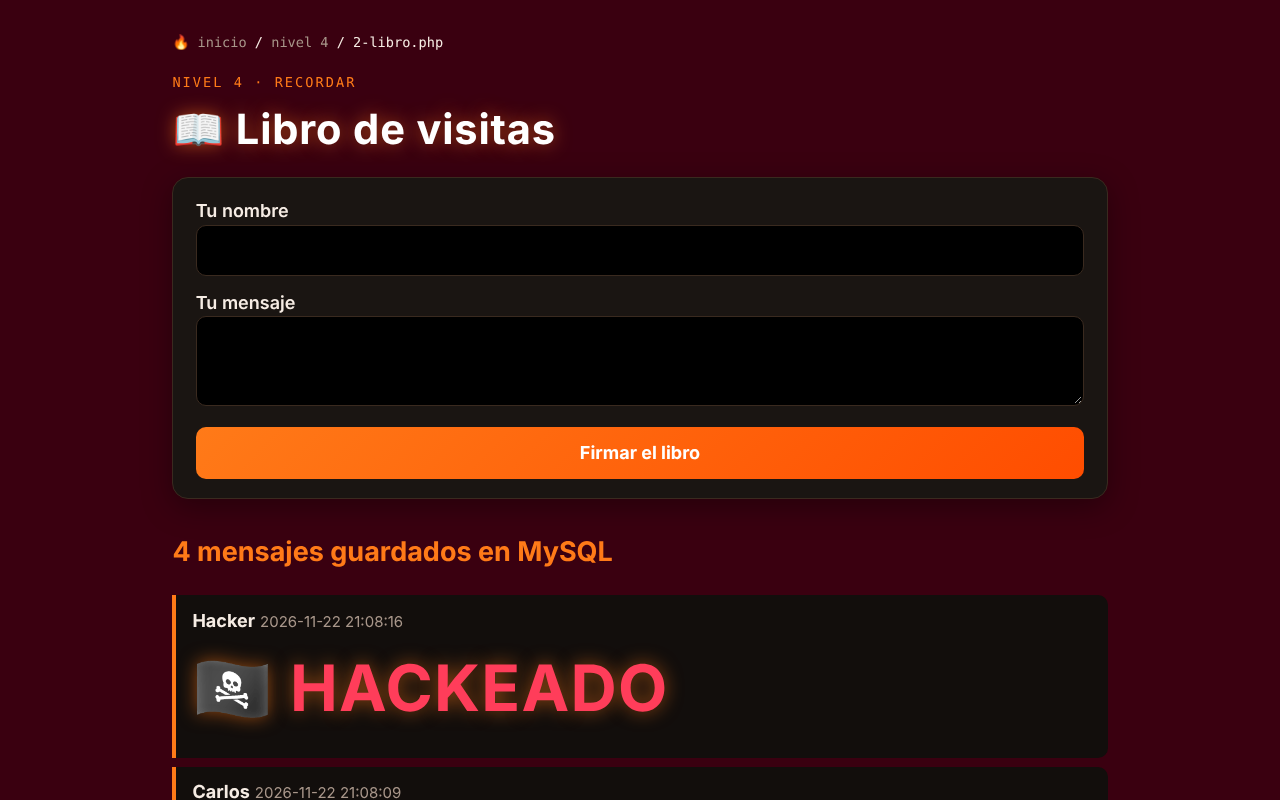
\includegraphics[width=11.2cm]{imagenes/libro-hackeado.png}};
    \node[anchor=south,text=texto,font=\large] at ($(current page.south)+(0,0.7)$) {Escribí un \textbf{mensaje}\ldots\ y \textcolor{brasa}{\textbf{cambió la página de todos}}.};
  \end{tikzpicture}
\end{frame}

\begin{frame}[fragile]{¿Qué acaba de pasar?}
\begin{columns}[T]
\column{0.52\textwidth}
\begin{codigo}[rojo]{lo que escribió el «hacker» como mensaje}
<h1 style="color:red">HACKEADO</h1>
<script>alert('hackeado')</script>
\end{codigo}
\vspace{2mm}
\begin{codigo}{2-libro.php · la línea culpable}
<?= $m['mensaje'] ?>
\end{codigo}
\column{0.44\textwidth}
\begin{dato}[brasa]PHP imprimió el mensaje \textbf{tal cual}. El navegador lo leyó como \textbf{HTML y JavaScript}\ldots\ y lo ejecutó.\end{dato}
\vspace{2mm}
\pause
\begin{dato}[oro]El Oráculo y el contacto \textbf{no} se dejan: usan un escudo, \texttt{htmlspecialchars}.\end{dato}
\end{columns}
\end{frame}

\begin{frame}[plain]
  \begin{tikzpicture}[remember picture,overlay]
    \llamas{-1.05}{-3.95}
    \coordinate (T) at ($(current page.center)+(0,1.1)$);
    \glitch[center]{T}{\fontsize{40}{44}\selectfont}{MAÑANA:}
    \coordinate (T2) at ($(current page.center)+(0,-0.3)$);
    \glitch[center]{T2}{\fontsize{40}{44}\selectfont}{HACKEÁ Y BLINDÁ}
    \node[text=texto,font=\large] at ($(current page.center)+(0,-1.55)$) {Inyección SQL · XSS · contraseñas · y tu proyecto listo para la defensa};
  \end{tikzpicture}
\end{frame}

% #####################################################################
%  CIERRE
% #####################################################################
\renewcommand{\hud}{CIERRE}
\begin{frame}[fragile]{PHP en una pantalla}
\begin{codigo}{todo lo de hoy}
<?php
$nombre = 'Ana';                        // variable
echo "Hola, $nombre";                   // escribir
if ($edad >= 18) { ... } else { ... }   // decidir
$menu = ['Saice', 'Ranga'];             // lista
foreach ($menu as $plato) { ... }       // repetir
$dato = $_POST['nombre'] ?? '';         // escuchar
require 'conexion.php';                 // abrir la despensa
$filas = $pdo->query('SELECT ...')->fetchAll();         // leer
$pdo->prepare('INSERT ... VALUES (?, ?)')->execute([$a, $b]); // guardar
\end{codigo}
\end{frame}

\begin{frame}{Ticket de salida}{3 minutos · en una hoja}
\begin{enumerate}\setlength{\itemsep}{3mm}
  \item ¿Dónde se ejecuta el código PHP: en el navegador o en el servidor? ¿Cómo lo comprobaste?
  \item ¿Qué diferencia hay entre \texttt{echo "\$precio"} y \texttt{echo '\$precio'}?
  \item ¿Para qué sirve \texttt{foreach}? Dá un ejemplo de tu proyecto.
  \item ¿Cuándo usarías GET y cuándo POST?
  \item ¿Por qué el libro de visitas se dejó «hackear»?
\end{enumerate}
\end{frame}

\begin{frame}[plain]
  \begin{tikzpicture}[remember picture,overlay]
    \coordinate (R) at (current page.center);
    \foreach \r in {1,2,3,4,5,6,7}{\draw[fuego,opacity=0.13,line width=0.6pt] (R) circle (\r);}
    \coordinate (T) at ($(R)+(0,0.8)$);
    \glitch[center]{T}{\fontsize{40}{44}\selectfont}{El fuego está encendido.}
    \node[text=texto,font=\Large] at ($(R)+(0,-0.45)$) {Hoy cocinaste tu primera página con PHP y MySQL.};
    \node[text=gris,font=\small] at ($(R)+(0,-1.9)$) {M.Sc. Ing. Juan Pablo Cruz Ovando · gerencia@jpcruzovando.com · jpcruzovando.com};
  \end{tikzpicture}
\end{frame}

\end{document}
